\chapter{Design of the Envoy File System}

This chapter examines the storage needs of service clusters and how they can be accommodated. Service clusters place specific demands on the storage system to efficiently support the deployment and management of untrusted services, but they also present helpful properties that can simplify the job. In addition to detailing these constraints, this chapter describes Envoy, a file system designed for this environment.

\section{Design objectives for Envoy}

Service clusters are a flexible platform for implementing arbitrary services, and the storage system that supports them must similarly flexible. While the design must not impose unnecessary restrictions on what clients are allowed to do, it can draw on expectations about how they will behave to guide optimizations. The high-level goal of Envoy is to predict and optimize for the most common client demands, while degrading gracefully as they stray from expected patterns. In addition, some specific requirements are derived directly from the needs of the environment.

\subsection{Running in a cluster}

Service clusters are centrally managed clusters of physical machines, each of which hosts any number of client services on private VMs. One of the chief advantages of using clustering independent services is that resources can be alloted based on average requirements even though many individual clients will be decidedly non-average. As actual demands are observed, the manager can periodically migrate running services to new hosts and redistribute the load to even out the combined demands of services on a single machine. To facilitate transparent migration, the storage system must not tie images to a single machine. Even private images used only by a single service must be location independent within the cluster, or capable of moving without forcing a restart or excessive disruption.

Incremental scaling is another important aspect of cluster environments. Using commodity hardware gives owners access to the best price to performance ratios, and building the cluster gradually in response to demand allows them to track the desired part of the curve as it evolves over time. The storage system must be capable of accepting new hosts without undue disruption to those already running. Note that unlike peer-to-peer systems \cite{blake} or networks of workstations \cite{anderson95a}, machines are under central control and are used for a single purpose, so machines coming and going is an exceptional event rather than the norm. Such events must be accomodated, but they need not be optimized for.

Another issue related to scale is that crash recovery must be localized. Transparent failover is not necessary, and recovering gracefully from failures rather than completely masking them \cite{baker94} is acceptable in this environment (note that hardware may fail as well; services that require specific reliability guarantees must implement redundancy at a higher level). Clusters are expected to run in machine rooms with well-provisioned machines that are properly managed, so failures are not expected to be frequent, but they are clusters of commodity hardware and failures will occur regularly for large installations. Confining the effect of a crash to a small area minimizes the damage, and restricting the disruption to participants with overlapping interests (sharing files, cache, etc.) is even better.

Besides imposing specific requirements, a cluster of commodity machines provides useful resources for designing a storage system. Commodity disks are big and cheap, and having them distributed throughout the cluster provides a natural source of distributed storage capacity. Machines may reserve some capacity for administrative use, for booting the machine, or for providing swap space for clients, but most is available for use by the storage system. These disks are not of premium quality, but can be expected to perform reasonably well. The disk can be no more available than the machine to which it is connected, so the storage system must provide redundancy across machines to tolerate failures. Since that cannot be avoided, combining disks into a RAID within a single node would only significantly increase the reliability of that node, not the system as a whole. Envoy assumes that disks are independent, and that the failure of a disk will disqualify the entire machine until it is fixed or replaced.

Commodity software is even more important than commodity hardware in supporting flexible commodity computation. By being presented with a choice of standard platforms and being charged according to how much they deviate from those basic starting points, most clients will be expected to draw heavily from common file system images. This can be considered a basic property of service clusters and the storage system must be designed to exploit it. Independent virtual machines introduce another scalar factor in scalability demands that could otherwise lead to excessive capacity requirements \cite{warfield}. This is mostly a benefit for the file system, however, because it allows Envoy to overlap caching even with unrelated clients.

\subsection{Supporting heterogeneous clients}

There is an inherent tension in service clusters between the goal of supporting the widest range of client applications possible on the one hand, while isolating them from each other and preventing unauthorized activities on the other hand. To address the latter concern, the storage system must be resiliant to arbitrary client behavior or misbehavior. Implementing the file system as a cooperative service run by the client would expose it to byzantine failures and considerable additional complexity. Instead, Envoy exploits virtual machine architecture to isolate the cluster-wide file system management from client code, just as individual clients are isolated from each other.

Combining file system functions at the physical machine level is not an arbitrary choice nor merely an artifact of using a virtual maching container. The host machine represents a new layer in the storage hierarchy that would otherwise be present on a cluster. Just as an operating system can aggregate the requests of unrelated processes, a file system manager can bring together the activity of all virtual machines hosted on the node, which may have no direct relationship or even awareness of each other. The failure of a client need not interfere with the continued operation of other clients or other machine-level nodes, and the vocabulary of the client is restricted to the protocol with which it connects to the file service, minimizing the damage that byzantine client failure can inflict on the rest of the system. The approach described here is not a requirement of the design, but the security and performance characteristics enabled can be considered minimum requirements for the intended use.

Containing and restricting clients is only one side of the struggle in service cluster design. The other part is providing services with as much flexibility as possible. For the storage system, this means that clients must have as much control over their file access as possible. Specifically, client operating systems must be able to both create and override their own file access restrictions. For private file system images, turning over complete control over access to clients would be sufficient, but arbitrating shared access to images by multiple clients requires a more hands-on approach. To support truly flexible scenarios, Envoy's security model must accomodate both.

Clients also vary in their longevity. Short-lived tasks will only thrive as part of the commodity computation ecosystem if they are cheap enough and can be deployed quickly enough to be competitive with the end-user owned and managed equivalents. Services that are tied to human activity may need to accomodate a human's impatience and short attention span. Interactive services or those that respond to other external conditions may need to expand over multiple instances in response to changing conditions, only to shut down excessive instances when a spike in demand subsides. These scenarios require a lightweight deployment mechanism that can rapidly produce not only standard base images, but also forked copies of custom file system images produced by clients. Forking running virtual machines is beyond the scope of this work, but file system support for the process is essential and relevant.

Long-lived clients have their own requirements, which must also be addressed in the storage system. Reliability can be considered a basic requirement of general-purpose storage systems, but additional support for backups and historical snapshots is also crucial especially for long-lived tasks. Runtime snapshots give a stable version of a changing file system image that can be backed up offline, used for reverting changes, examined for debugging purposes, or analyzed for forensic purposes after a service has been compromised. Only clients can determine the right tradeoff between the extra storage costs invoked by snapshots (which retain files that would otherwise be deleted) and the convenience of a detailed history, so Envoy must allow each client to dictate its own snapshot policy.

Envoy must be able to provide a private, bootable image for each service that launches. Platforms for embarassingly parallel problems and other homogenous service platforms can install basic software at each node and rely on a shared file system only for shared data. The profile of service clusters admits this possibility for starting the virtual machine manager and other administrative software, but individual services cannot be tied to a specific machine. Even the possibility of supplying a range of standard base images on each node and using a stacking file system to export virtual private images falls apart as clients fork highly-customized images, leading to inconsistency and excessive management complexity. A better solution is to require that the storage system be able to supply globally accessible images and location transparency, but do so in a way that accomodates the common case (many private images used by a individual services that migrate infrequently) with good performance. The convenience of global accessibility and transparent mobility must not cost much when it is not used much.

Service clusters are a platform for flexible commodity computation, which may take the form of distributed services as well as self-contained computation processes. Private images may be the most common case, but transparent file sharing is just as necessary for larger services. This leads to the problem of controlling shared access as mentioned above, and also to the necessity of managing concurrent file access. Past studies have repeatedly concluded that runtime contention is quite rare, but the potential is always present in a shared file system. Envoy aims for perfectly consistent file sharing, i.e., any read performed after a write completes observes the full effects of that write, and it does so with the further requirement that scaling of shared images be limited only by the extent of overlapping access. Subsets of a shared space that are used by only a single client should perform like private images, again supporting a range of access patterns but optimizing for the most common case.

\section{Using Envoy}

\subsection{Basic environment and assumptions}



It's a cluster, dom0 is trusted, it's all managed together, expect users to start from standard installs

\subsection{Use and administration}

This section presents the administrative interface to Envoy, which is designed as a series of special file operations and conventions.

All services share a single cluster-wide namespace tree with a common root. Mounting the root of the entire tree requires special priviledges, normally reserved for the administrative tools managing the file system. The top levels of the hierachy respond normally to standard file operations, with a few notable exceptions described here.

A few file names are given special significance and their use is restricted. The name \current is reserved for use as the root of a client file system, positive integers are reserved as the read-only roots of snapshots (in ascending order) of the tree rooted at \current in the same directory, and a symbolic link names \snapshot is created and protected by the system to link to the most recently-created snapshot in the same directory. In addition, a normal file named \password can exist to store credentials for clients accessing descendents of the containing directory.

The namespace is conceptually divided between the administrative levels and the client levels. The client levels include anything that is a descendent of a directory named \current or one of its snapshots (named as positive integers). Any path that does not pass through one of these points is considered part of the administrative namespace and is subject to the restrictions and special semantics described in this section.

To create a new file system root, a user or management tool creates any desired layers of files and directories within the administrative area, ending with a directory called \current. Services can then mount \current or any of its descendent directories. A client mount request specifies the desired root pathname along with the username attempting the mount and any credentials required to validate the request. The server checks these credentials against any files called \password that it encounters in administrative directories passed through before arriving at \current, with those further down the hierarchy overriding those encountered earlier.

In addition to end-user mounts, this system of password files applies to the administrative file areas as well. If given suitable credentials, a service can attach to the namespace in an administrative directory to create and manage its own file system trees and credential files, creating a hierachy for management roles as well as file storage. Controlling access to any directory requires credentials to mount its parent, along with standard file permissions within the parent directory to manipulate the credential file. Envoy does not map user and group names to numeric IDs, so any clients that can agree on usernames and credentials can share access to a file system.

The \current directory---in addition to marking the transition from administrative to client directories--- can have its snapshot taken. When the server receives a request to create a symbolic link with a positive integer as its name and \current as its target, it checks to make sure that the integer is correct for the next snapshot (either \texttt{1} or the number linked to by \snapshot plus one). If so, it takes a snapshot of \current, makes it accessible using the requested name (accessible as a directory, not a symbolic link), and creates or updates \snapshot to link to the newly created snapshot. Any request with the wrong target or the wrong number is rejected.

Snapshots are always given positive integers as names (and cannot be renamed), but this is not always convenient for use. It may be useful to name a particular snapshot with a more meaningful name using a symbolic link. Symbolic links are normally considered opaque by the server and cannot be used in any mount or directory-change requests, so to make accessing named snapshots more convenient the server silently dereferences symbolic links that refer to snapshots in the same directory.

Snapshots also serve another special purpose: they can be used as the root for a file system fork operation. Just as the \current directory diverges from its most recent snapshot using copy-on-write semantics, new \current roots in other administrative directories can use an existing snapshot as a starting point. A request to create a symbolic link called \current that refers to the fully-qualified pathname of a snapshot (again, links to a snapshot within the same directory are dereferenced, but others are not) is treated as a fork operation using the given snapshot as the starting point for a new root file system. The newly forked file system is subject to the same rules as those created with \texttt{mkdir}, and respects the credentials local to its creation site, not those of the snapshot from which it diverges. For this reason, fork operations require sufficient credentials at both locations.

\section{Architecture}

Services access Envoy using a client-server network file system interface. Each physical machine in the service cluster runs an administrative virtual machine that manages the storage processes for all services on that machine. The services on this VM partition the local disk between a constribution to the shared storage pool and the local persistent cache as well as providing a standard interface allowing other hosts on the machine to access the file system. \prettyref{fig:single-machine} illustrates a typical machine. By giving clients access to the system through a proxy on a trusted VM, they can use simple, well-understood client-server access protocols to join a more complicated system \cite{shapiro}. Byzantine failure from clients is less of a problem, because they have a limited interface to the system and hold no trusted data.

\begin{figure}[tp]
\centering
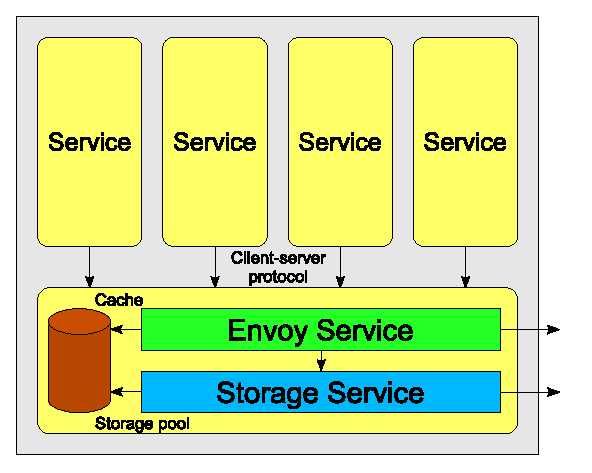
\includegraphics{figures/single-machine}
\caption{Each physical machine has a single administrative VM that hosts the Envoy services. This VM exports a network file system protocol to other service VMs running on the same machine.}
\label{fig:single-machine}
\end{figure}

The file system management processes join a cluster-wide service that is comprised of two primary layers, as illustrated in \prettyref{fig:layers}. Storage is managed by the lower level, which allows a small set of basic file operations on objects. All operations are stateless and the storage service makes no attempt to prevent or manage concurrent requests or to enforce any kind of security policy. Objects are extents of bytes with a small set of attributes.

On top of the storage service is the envoy layer, which builds a hierarchical file system out of objects, coordinates access to files, provides authentication and access control services, manages caching, and exports a standard network file system interface for services to access.

\begin{figure}[tp]
\centering
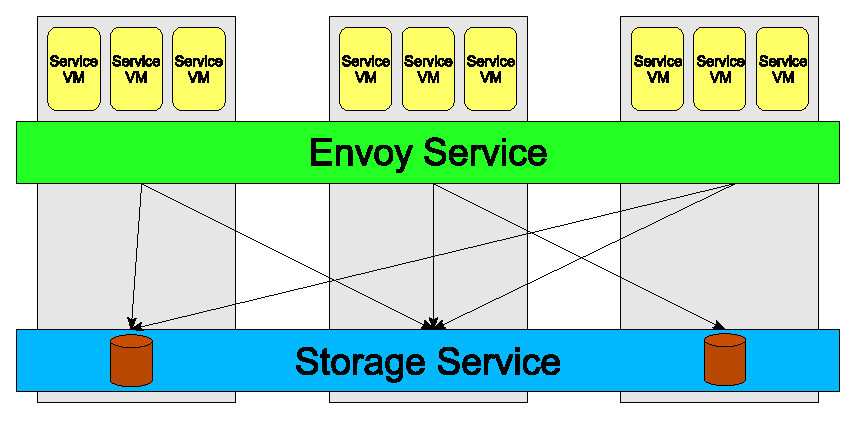
\includegraphics{figures/layers}
\caption{The envoy service coordinates access to provide a single, coherent view of the distributed file system. It relies on the storage service, which provides a repository of objects referenced by unique identifiers.}
\label{fig:layers}
\end{figure}

In the remainder of this section I detail the functionality and requirements of these systems and consider the tradeoffs of various design decisions.

\subsection{Distribution}

\prettyref{fig:client-server} depicts a commonly-used storage arrangement using a series of dedicated file servers to handle the needs of many clients. This architecture is successfully used in many settings and, despite alternatives developed over the years, is still the dominant storage model in practical use.

\begin{figure}[tp]
\centering
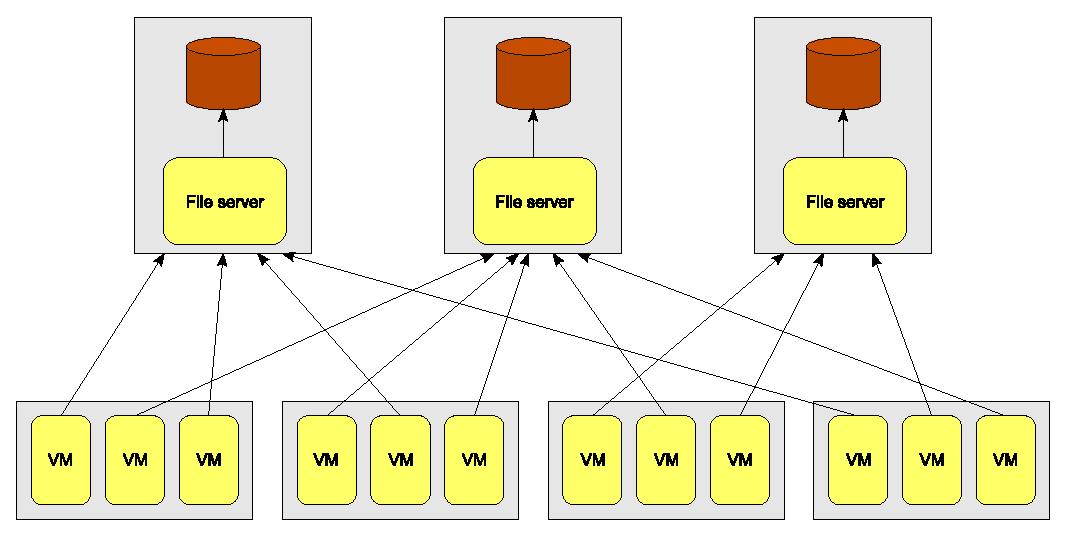
\includegraphics[width=100mm]{figures/client-server}
\caption{A popular storage solution for groups of clients involves a series of dedicated servers. Content on the servers is carefully managed to distributed storage demand and transaction load between the servers.}
\label{fig:client-server}
\end{figure}

The client-server model has obvious flaws when applied to clusters with many transient clients. Data placement decisions must balance space requirements and expected access rates in order to avoid overloading a particular server. Rebalancing---a disruptive and time consuming job---may be necessary in response to added clients, added servers, added disks, variations in client workload, and accumulation of data over time.

With the service cluster model, the problem is made even worse. To make efficient use of increasingly powerful hardware, each physical machine may host many services, each of which requires a boot image as well as access to the data relevant to its intended task. Dividing each machine means that there may be an order of magnitude more virtual machines than physical machines, putting excessive demands on a centralized storage infrastructure \cite{hospodor}. Single-purpose services may also be short lived or vary by time of data, making manual balancing impractical.

The client-server model has not endured as long as it has simply for lack of alternatives, however. It has many strengths that can inform the design of a more distributed architecture. With a single server managing shared data, concurrent access can be managed simply through explicit leases and cache invalidation, centralized caching with synchronous access, or through a lock manager. Whatever the mechanism for resolving conflicts, a centralized server is ideally suited to detecting and responding to concurrent requests because it is the point on the access graph at which all requests converge. The consistency of data that has reached the server is as good as its backing store.

The simplicity of a server is also a virtue. A failstop model for reliability can generally be assumed, backups are relatively straightforward, the server is typically dedicated to a single task or is shared with other trusted services, and the semantics are simple to define in terms of client behavior%
\footnote{NFS versions 2 and 3 have notoriously complicated consistency semantics, but this is almost entirely due to client policies. NFS server semantics are straightforward.}.

The chief faults of a centralized system are the introduction of a single point of failure and the inability to scale beyond the network and disk bandwidth that can be hosted by a single server. While these limits are unacceptable at large scales, they are quite servicable for small groups of clients.

For clients that are sharing data, it is difficult to improve on a centralized server. For sufficiently overlapping data sets, any consistent model will degrade to something resembling a server during periods of contention because all interested clients will have to synchronize their access to the contended bits. A single arbitrator will ultimately oversee each bit of data, whether it is a traditional server, a lease-holding client, or a quorum of cooperating peers.

Sharing cache space is also a benefit of consolidated control of shared data. As the performance gap between disk access and memory access continues to grow, efficient use available cache space becomes increasingly important. Once again, a single centralized cache fails the scalability requirement, but a shared cache for a smaller set of clients with overlapping data needs provides attractive properties. Accessing a cache across a high-speed network is faster than accessing a local disk \cite{dahlin94b}, so in a cluster setting, organizing the aggregate cache around shared access patterns is more valuable than organizing it to localize access. Stated another way, the combined effective cache size of the entire cluster is greater when redundant entries are consolidated through sharing, and maximizing the combined cache size to avoid disk seek penalties is becoming more important than avoiding the network hops that arise from using a shared cache.

While a server cannot handle an unlimited number of clients, it can serve many clients under typical workloads. Scalability matters more at the level of the entire distributed system than when considering individual nodes. In the case of overlapping requests from different clients, a shared cache on a shared server will outperform a series of private servers, despite the overhead of network latency. Given that runtime contention is relatively rare \cite{kistler}, Envoy is designed to localize file ownership when there are no apparent conflicts, but to pick one participant to own files that are shared and act as a server to the others.

This principle of localizing control where possible, but reverting to a simple, well-understood client-server model when sharing is necessary is fundamental to Envoy. It leads to \emph{fate sharing} amoung clients with overlapping interests in the areas of performance, resource usage, and failure recovery. In each case, services with overlapping resource demands cooperate directly with each other and disinterested parties are not involved.

The overall distributed architecture of Envoy is modeled after human-administered systems using client-server file systems. Storage is distributed over a series of servers in an attempt to balance demand (the seperate storage layer handles balancing capacity), but where a human administrator is constrained by practical concerns to using relatively few, well-provisioned servers, an automated system can continue the process of server division and balancing to a much more fine-grained level. Entire images or parts of images that are used exclusively by a single service (or a group of services hosted on a single physical machine) are managed directly by the envoy service on the same machine. Where sharing occurs, the client with the highest demand retains direct control and acts as a proxy for other clients accessing the same storage, thus sharing a cache and avoiding complicated coordination protocols.

\subsection{Storage layer}

Citations: \cite{stein05}, HP trace shows that with caching, most operations that go to disk are writes, and non-sequential operations \cite{ruemmler}, so access patterns are probably less important in the storaage layer than recovery concerns, which pimp for chained declustering and correlated failure \cite{lee96}. Object storage works well and is growing in popularity \cite{factor}. File layout doesn't matter as much behind the cache \cite{stein05}

The objective of the storage layer is to provide a simple, stateless interface for accessing objects. Redundancy to enhance availability and reliability and distribution to balance load is also handled by this part of the system. The storage layer is implemented in two parts, called the top and bottom halves.

The bottom half is implemented in the storage daemon hosted on each physical server. While the storage daemon instances form a collective pool of storage, they do not communicate directly with each other. At the local level, each storage manager is unaware of any global state, and responds blindly to incoming requests from the envoy layer. Instances do not attempt to balance load, resolve conflicting requests, or create redundancy, nor do they monitor which object IDs they considered valid. Instead, they provide a thin, simple storage service for numbered objects with attributes.

To make these servers more useful, the top half of the storage layer is implemented in the envoy daemon. It is responsible for mapping an object ID to the set of storage server instances that host the referent object. Combined with the persistent cache, the storage layer top half provides a simple procedural interface to the storage layer, where objects are named by unique IDs. The top half is responsible for creating and locating replicas, detecting and masking/recovering from failures, allocating new object IDs when needed, and reading and writing data and attributes.

Numerous strategies are available for distributing objects across the cluster. While I discuss some of them here, I only do so with the intent of demonstrating that an independent storage layer is viable and reasonable; many other object storage systems of varying levels of sophistication could be substituted for one I describe and other work has addresses object storage in more detail than I attempt here. The emphasis of this dissertation is on the envoy layer as implemented on top of the object layer.

\subsection{Envoy layer}

The envoy layer forms a file system from the objects provided by the storage layer, coordinating and caching access to the file hierarchy, and exporting a client-server protocol to services that act as clients of the file system. The entire cluster shares a global, hierachical namespace, but clients typically mount a subtree from the hierarchy and treat it as a complete file system.

\subsubsection{Territories}

A single instance of the envoy service runs on each physical machine. The global name hierarchy is divided amoung participating instances in the cluster. When a given instance takes responsibility for some part of the namespace, it is said to \emph{own} a \emph{territory} covering the relevent subtree of the hierarchy. All operations within local territories are served locally and may be cached locally both in memory and in the persistent cache, which is reserved exclusively for territories local to the machine.

This partitioning of the global namespace and the resulting federation of constituent parts is what gives Envoy its name. When clients request operations that stray from the local territories, the requests are handed off to the envoy on the appropriate machine. It follows that each instance must know not only the boundaries of its own territories, but how to find the envoy for neighboring territories, i.e., those that can be reached by a single directory traversal (up or down) from a local territory.

The envoy service is stateful, and tracks not only its territories and neighbors, but the state of all files and directories in use by its client services. When a client navigates beyond the boundaries of a local territory, requests are forwarded directly to the owning envoy. If further navigation moves beyond the neighbor's territories, the neighbor does not forward it to the new envoy, but instead bounces the request back to the originator with the address of the envoy that can answer the request.

Under this system, two envoys maintain a direct relationship with each other only when they are immediate neighbors in territory ownership, or when one is serving requests for a client of the other. It follows that if territories are alloted such that the owner of a territory is also its most active user, traffic on an envoy instance will generally be dominated by its local clients.

Often, the best that can be achieved in a steady-state system is to have the owner of a territory be the envoy driving a plurality of traffic, not a majority. Sometimes this is an inevitible consequence of overlapping client demands, but often some further gerrymandering of the territory boundaries can restore a majority to the local territory. Since the needs of the clients and the needs of the envoys are generally aligned, a practice that in polotics usually serves those in power at the expense of those they represent serves both equally well in file systems.

\subsubsection{Files}\label{sec:directory-format}

Files and directories can be mapped easily to objects as provided by the storage layer. Files are stored as objects with a set of attributes, and directories as files with special semantics and a different interface. Certain special files are stored as normal files with special contents, accessible through the interfaces appropriate to the file types.

Unix file systems are organized around \emph{inodes}, which encapsulate the contents of a file with its attributes, but not with its name. Envoy employs a similar structure, with file contents and attributes seperate from the name hierarchy. Objects also have numeric identifiers like inodes, but it is worth noting that these identifiers can change during the lifetime of a file, so an object ID is not suitable for identifying a file.

Directories are files containing listings of other files. In Envoy, directories are managed at the block level, with each block containing some number of entries. An entry consists of a file name, the object ID that links to its contents and attributes, and a flag indicating the file's copy-on-write status. When this flag is set, the object is considered read-only, and will be cloned before any changes are committed to the file's contents or attributes. This process is completely opaque to clients.

Special files, such as device nodes and symbolic links, are stored as regular files whose contents follow a defined format. For symbolic links, the file contents are the target of the link, for devices they are an ASCII string identifying the major and minor device numbers, etc.

\subsection{Caching}

Citations: Most files in a file system (90\%) are never accessed after being created and as few as 1\% are used daily \cite{gibson98b}, so even a small persistent cache can be effective, and sharing the active files from boot images and the like will probably see heavy overlap: after all, moving only 1,000--10,1000 objects takes 42--77\% of the load with it \cite{klosterman} (reconcile this with \cite{muntz}). Another workload comparison \cite{roselli}. DBMS work also explores the idea of considering the aggregate cache capacity of the client-server system \cite{franklin}. Self-similarity in file systems \cite{gribble}. Speculative execution has been used to mask the latency of distributed file systems \cite{nightengale}, allowing improved performance without sacrificing cache consistency, and approach that compliments ours. Other work on consistency \cite{triantafillou,vilayannur}.

The cache design in a distributed file system must balance the needs for performance, consistency, and durability. While maintaining a coherent view of the file system that is tolerant to software and hardware faults, a cache should reduce latency, increase throughput, and increase overall capacity by reducing the network and disk congestion required by a given amount of activity and freeing input/output channels to absorb additional load.

Enhancing performance is the primary reason for employing a cache in the first place. The growing gap in performance between main memory and disk makes effective cache management critical, as a random disk access is five or six orders of magnitude slower than a similar memory access. Much work has been done exploring different cache replacement strategies, with significant gains to be had when future traffic can be predicted. Unfortunately, the service cluster environment does not provide any insight into the expected access patterns of its constituent services, as one of the purposes of the environment is to support arbitrary services.

In a 2002 interview \cite{spring}, the CEO of Google observed that for seek-intensive workloads, DRAM can be cheaper to deploy than disks. The seek time of a single disk cannot be improved significantly, so increasing overall disk performance generally requires adding redundant spindles. With many mirrored disks, many seeks can proceed in parallel and a random request can be satisfied fastest by the disk whose head position happens to be nearest the requested datum. Because the of the large performance gap, Google found it cheaper and faster to store their entire web search index in DRAM, which can serve many requests quickly, than to create enough replicated disks to handle the same transaction load.

While Google's implementation revolved around an inherently parallel task, it can still inform the design of a cache solution for Envoy. A single, commodity machine cannot hold as much memory as would be required for an index of the web, but by considering the aggregate capacity of a cluster instead of focusing on the capabilities of a single machine, they arrived at the suprising but sensible conclusion that ``it costs less money and it is more efficient to use DRAM as storage as opposed to hard disks''. Finding data in a local cache is ideal, but with a high-speed network connecting machines in a cluster, it is faster to query the cache of another machine than a locally-attached disk \cite{dahlin94b}, suggesting that it would also be prudent for the design of Envoy to consider the combined cache of the cluster as well as the cache of individual nodes.

Envoy is designed to compromise between the competing goals of maximizing local cache hit rates and maximizing the aggregate cache capacity of the cluster. Two design features are particularly relevent to addressing these goals. The first is that all client requests are served synchronously by the envoy service without the aid of a local cache. Instead they rely entirely on the shared cache hosted by the envoy service in its private virtual machine. The local envoy directly services all requests---local and remote---for territories it owns, so the entire cluster caches at most a single copy of a given file.

This could potentially strain the envoy that owns a particularly popular file, as it funnels all traffic for that file to a single node. For light to moderate sharing, this is not an issue, and in practice the envoy will be accessing the file mainly from its cache and can handle significant traffic. For extreme instances of sharing, I argue that services should use explicit network-facing protocols instead of relying on the file system as a \emph{de facto} distributed shared memory system.

The second design feature has a more complex impact on the aggregate cache capacity. Territorial boundaries are drawn along boundaries in the namespace hierarchy, but because of the copy-on-write mechanism in snapshots and file system forking, multiple names may refer to the same underlying storage layer object. This only happens when the object (but not necessary the file) is read-only, so cache consistency needn't be considered, but it does mean that multiple envoys may cache the same underlying object. While this mechanism introduces redundancy in the cluster-wide cache, it also has the potential to consolidate cache entries within a single envoy instance. If multiple services are using different files backed by the same object, they will occupy the same place in the persistent cache as well as the in-memory cache.

Cache utilization is most effective when clients on a single machine use file system images forked from a common root, and the more complete the root image the more likely it is that services will rely on common rather than custom-installed files. This fits nicely with the stated goals of flexible commodity computation, where both the host and the client gain from using the most popular commodity tools. The host by reducing client footprint and increasing capacity, and the client by reducing deployment costs and maximizing performance through increased cache hits.

\subsection{Data paths for typical requests}

To summarize the architecture of Envoy, consider the data paths followed by typical file system requests as depicted in \prettyref{fig:hops}. The best case (retrieval from in-memory cache on the same machine) is designed to be the most common, with extra steps being required in progressively less-common operations until the worst case, where a request travels from a client to the local envoy service, is forwarded to a remote envoy, misses the local cache and is forwarded to a storage server instance where the data is retrieved from disk.

\begin{figure}[tp]
\centering
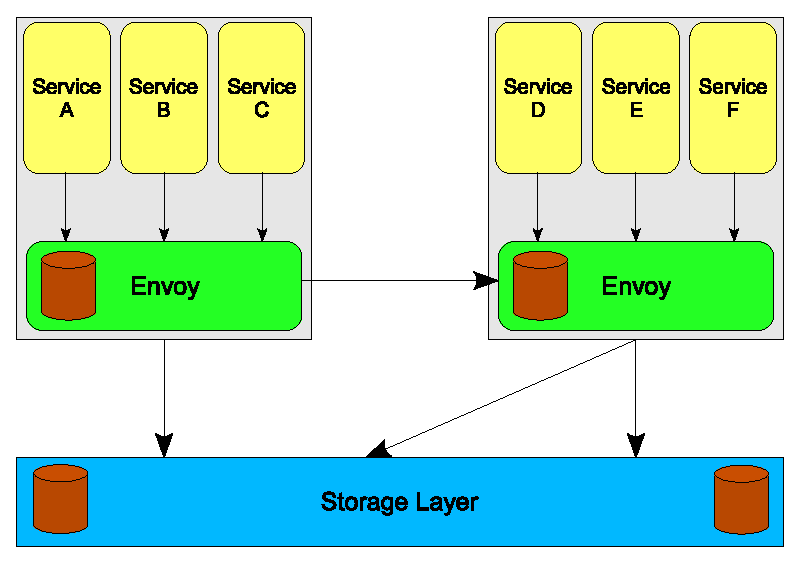
\includegraphics{figures/hops}
\caption{File system requests proceed from service VMs to the local envoy service. A request from a local territory may be filled by the local in-memory cache, the local disk cache, or by a single network hop to a storage server. A request for a foreign territory adds a single network hop in each case, as the local envoy acts as the client to a remote envoy.}
\label{fig:hops}
\end{figure}

\subsubsection{Read operations}\label{sec:data-paths-read}

The best case is a request for hot data in a local territory. In this case, data can be served from the in-memory cache of the local envoy server. With a fully optimized implementation using Xen or a similar VM environment, this data transfer can occur with a single data copy from the cache to a data page, and that page can then be swapped directly to the client VM via page table manipulation. Since the client's OS does not keep a cached copy, that page can likewise be passed on directly to the client application. While my prototype is not this optimized, the design permits a very lightweight operation involving a single data copy and some metadata manipulation.

Warm data from a local territory follows a similar path, prefaced by retrieving the requested data from the local persistent cache (on disk) into the in-memory cache. With large, cheap commodity disks, the persistent cache can easily hold several operating system images and typical application suites. Typical Linux installations occupy no more than a few gigabytes, and even that includes many supporting files that are rarely used and may never be referenced in common service deployments. If services have forked from standard base images as proposed, it is realistic to assume that the entire operating system and standard applications will be available in the local cache hierarchy for a service being deployed on an active node.

When the local cache fails to deliver, the envoy service must retrieve requested data from the storage layer. The top half of the storage layer provides a complete object server catalog, so a request can proceed in a single network hop to the node in the storage layer bottom half that hosts the needed object. For simplicity, the persistent cache holds only complete objects, so an entire object must be transfered before the envoy service can begin fulfilling requests from the local cache. If the object is replicated, the envoy stripes the transfer across the servers, e.g., if there are three replicas, it streams the first third of the file from the first server, the middle from the second server, and so forth.

Operations in territories outside local control add an extra network hop between the local and remote envoys for all operations. The data also bypasses the local cache, so locality of reference does nothing to remove this network penalty. It does offer another optimization opportunity (the data, once received from the network, can be passed to the client application without any further copying) but this is minor compensation for a guaranteed latency penalty.

Fortunately, this penalty need not be too great nor too common. The remote envoy handles the request just as it would one from client local to it, including caching, so referential locality does improve performance from the cold-cache worst case. The target environment is service clusters, too, with high-speed local area networking and unmetered inter-node traffic. Finally, because of the way territories are decided, in a steady state system foreign envoy requests generally imply some degree of sharing. While relatively uncommon in itself, genuine sharing requires \emph{some} form of synchronous network communication to guarantee consistency, so Envoy's goal of reducing synchronous inter-node to cases of either sharing or infrequent access seems a reasonable one.

\subsubsection{Write operations}\label{sec:data-paths-write}

Citation: Transactions, strengths and weaknesses \cite{gray81}.

Write operations are less common than reads, but much of the complexity in file system design comes from supporting them. While a good cache satisfies many read requests from memory quickly and with no correctness concerns (provided coherency is maintained in the case of distributed systems), write operations cached in memory raise concerns about durability. If the server acknowledges the write operation as being complete but has only committed it to an in-memory cache, then there is a window of vulnerability before the data is stored to disk and all metadata updated wherein a system crash could lose data that the client expects to be resilient to crashes. In an isolated client, this may be acceptable as the client will simply be forced to restart from the state that was committed to disk and will generally only lose a boundable amount of work. It is particularly problematic for distributed systems and others with external side-effects, however, where other participants may cue subsequent actions on the premise that a write has been successfully and durably committed to disk. The problem is further exacerbated in a commodity hardware environment where failures are routine.

At the other extreme, one can commit all writes to disk before completing the transaction. This makes it clear to the client when a write operation has been consumated, and it is free to either wait for the acknowledgement or proceed asynchronously with explicit knowledge of the risk it is assuming. While this is a simple and appealing model, it ignores two important realities. The first is that the default action for most commodity operating systems is to cache writes and acknowledge them immediately while delaying the disk write. Changing the expected performance characteristics of a basic operation like writing to disk would not provide a commodity-friendly environment as it would severely affect the perforamnce of many standard tools in a negative way. The second is that most files created are short-lived temporary files that are soon deleted \cite{ousterhout}, so synchronously writing them to disk introduces not only unnecessary latency but also unnecessary disk contention.

Several intermediate possibilities exist. Instead of having write requests proceed directly to the storage layer, the local persistent cache could be used as a staging area, with write requests being committed locally and then forwarded to the storage layer after some delay. This would do little to improve performance, however, as synchronous disk access is slower than synchronous network access, so this would not eliminate the slowest link in the event chain. Specialized hardware with involatile memory could also act as a staging area, giving good write performance while retaining durability. The latter approach violates our goal of using widely-available commodity hardware, however, and neither approach is resilient to hardware faults that result in the entire node failing.

Another approach is to only guarantee synchronous durability when explicitly requested by the client, using the equivalent of the Unix \texttt{fsync()} system call. This matches the semantics of local file systems, and thus what most software is written to assume. It is not without faults, however, as the popularity of high-level scripting languages and middleware frameworks (especially for network services, exactly the types of clients service clusters are designed to support) means the connection between application actions and disk operations is often obscured. Requiring low-level controls to get correct behavior is often an acceptable compromise, but it is rarely ideal.

The solution Envoy employs is based on exploiting the cluster environment. While commodity hardware is expected to fail occasionally, simultaneous failure of multiple machines is still relatively rare, provided that the nodes are sufficiently isolated from each other in terms of power and cooling. Since service clusters are intended for professional hosting environments, it is reasonable to assume that hardware faults occur in isolation. With that assumption, durability is less about committing data to disk and more about rudundancy. A write request is considered final when it is in the memory of all of the storage servers that will eventually commit it to disk. If the envoy server fails, the storage servers are unaffected. If one or more of the storage servers fails before committing the data to disk, the recovery mechanism must restore consistency using the most up-to-date of the replicas. Having storage servers potentially out of sync due to a failed asynchronous write in this scenario is fundamentally no different from having one fail while trying to satisfy a synchronous request. In both cases, the inherent asynchrony of the network means that only the degree of the problem changes.

\section{File system images}

A single, hierarchical namespace unites all the participants in an Envoy cluster, but for management purposes there are two distinct levels. The administrative file tree starts at the root of the namespace and has as its leaves the file system \emph{images} that are normally accessed by clients. Imposing this additional structure in the tree codifies the intended usage pattern, which simplifies administration and allows for some simple but effective optimizations.

\subsection{Security}

Service clusters must accomodate a heterogeneous collection of clients, some of which may trust each other, but most of which will not. To support standard operating systems and tools, Envoy must support familiar semantics, including granting complete control over private images, while also accomodating shared images that grant limited access to various clients.
\note{TODO}

\subsubsection{Enforcement}

Envoy is designed with a fail-stop failure model. This is relatively simple to deal with, but is unrealistic in many environments. Service clusters 

Envoy services run in trusted virtual machines that are administered by the owner of the cluster. Messages from one envoy to another and to storage servers must be authenticated to ensure , either by  
\note{TODO}
\subsubsection{Policy}

Access to images is controlled through \texttt{password} files in the administrative directories. At the time a client mounts an image, its credentials are checked against all password 

\note{TODO}

\subsection{Forks and snapshots}

A few additional rules simplify management. The root of the namespace is always writable, as are all administrative directories, i.e., those that are not descendents of a directory called \current or one of its numbered snapshots. Snapshots are always immutable

\subsection{Deleting snapshots}

Storage space is cheap and plentiful, and systems such as Venti are designed to keep a complete history of all files ever created \cite{quinlan}. This may be appropriate for some workstation environments, where the increase in storage capacity can outpace typical data creation rates, but deleting files permanently is still a necessity for many other users. In service clusters, users are charged according to the resources they use, so they must have the flexibility to completely remove old files. Also, when clients leave a particular service cluster, the owner may wish to reclaim the space for future use, as there is little incentive to keeping it around on behalf of a client that is no longer paying. Also, concern for privacy and complience with data retention laws may require data to be completely removed.

Backups in Envoy are done through snapshot operations, and anything created and deleted in the window between two successive snapshots is no longer accessible anywhere so it is deleted immediately (with an exception described in \prettyref{sec:hard-links}). This is easily detected through the copy-on-write mechanism, which identifies all files that were created since the most recent snapshot. All files with copy-on-write flags (either explicit in a directory link or implicit through an ancestor's link) are backed by objects referenced by one or more read-only snapshots, so envoys never delete these objects when their corresponding files are deleted.

The problem comes when trying to delete old snapshots, as it can be difficult to determine which storage objects are used only by the files in a given snapshot.

One obvious solution would be to implement reference counting in the storage layer. This has the advantages of simplicity, accuracy, and immediacy. The main disadvantage is that it puts the performance burden in the wrong place: every time a directory object is cloned (an frequent operation after a snapshot as the copy-on-write mechanism supports write requests) the reference count for all objects in that directory would need to be incremented. This would require clone operations to be implemented in the envoy layer which can locate all object replicas, or the bottom half of the storage layer (where clones are implemented) would need to be aware of the topology of the entire storage layer, a requirement currently confined to the top half. In either case, a lot of extra traffic would be generated to support an operation that is relatively infrequent and not timing critical.

The copy-on-write mechanism in Envoy is similar to the one I implemented while working on Parallax \cite{warfield}, as is the problem of deleting snapshots. The problem was simpler in Parallax, however, which uses a copy-on-write radix tree to map logical blocks to physical blocks in a virtual block device. The virtual block numbers do not change between snapshots, so comparing the physical blocks mapped to by two successive snapshots reveals which blocks from the first were unlinked during the lifetime of the second.

With Envoy and its hierarchical file tree, the problem becomes more complex. Comparing two successive snapshots is no longer straightforward, because files and directories can be renamed. The virtual block IDs that are static in Parallax are replaced by variable names in Envoy, making the process of comparing two snapshots more difficult. Supporting hard links makes it even more difficult to define a one-to-one correspondence between object references in two successive snapshots.

This potentially messy problem can easily be solved by brute force. Instead of imposing extra runtime overhead for normal file operations or attempting to walk two file systems and identify matching files within them, it is simple and practical to gather a complete list of objects referenced by an image. Using 64-bit object IDs, such a list would take 8 megabytes for every million files. In a 1999 study of workstations at Microsoft, Douceur and Bolosky found an average of 13,309 files over 10,568 machines, with the subset running NTFS (the newest file system studied and the one with the largest average number of files) averaging 24,229 files over 3332 machines \cite{douceur99}. This number will no doubt continue to grow, but anecdotal tests found the number still in the low millions for typical, modern Linux desktop installations.

Just as high-level languages are worth using despite being slower and using more memory than lower-level languages, I consider the simplicity of gathering a complete list of objects and sorting it to outweigh any potential performance loss compared to a more sophisticated but more complex approach. For problems like this one, it is not even the relative performance or storage requirement that is salient, but the absolute size: deleting snapshots is not a critical path operation and for typical image sizes the brute force approach is cheap enough that no amount of optimization would be worth more than a very small complexity increase (Amdahl's law \cite{amdahl} is relevant here, but the ability to execute the operation asynchronously makes any (reasonable) cost even less important).

A sorted file with all object IDs referenced in the snapshot can easily be stored in the administrative directory that contains the image. To delete a snapshot, the objects of it and its immediate successor and predecessor are compared in order. Each object that appears in the snapshot but disappears in the successor can be safely deleted from the storage layer. To make it safe and resilient to crashes, the envoy service ensures that no clients are currently accessing the snapshot, then it unlinks the root of the image first, and deletes the list of object IDs last. At recovery time, an object ID file found without a corresponding image indicates that a crash occurred before the operation completed, and it can be safely restarted. The image itself isn't necessary at this stage, and as long as the cleanup process can tolerage objects having already been deleted, it can work entirely from the object lists.

The only other complication in this process is image forks, where multiple successors may exist for a single snapshot. Forking an image does not directly affect the snapshot used as the starting point, so the easiest way to detect forks it to log them. The log is consulted before any snapshot delete attempt, and deleting images that have more than one immediate successor is not permitted.

A few other corner cases are worth mentioning. The current version of an image can be deleted using the same procedure, but it must be made read-only or client access must be disallowed before gathering the list of object IDs (note that access is normally only forbidden when deleting starts, as the catalogs of predecessors and successors must be assembled as well as those of images marked for deleting). Otherwise, the normal procedure suffices, with the successor object catalog taken to be empty. The log of image forks also needs to account for deletes, so that entire trees of images can eventually be pruned back to the root if desired.

\section{Dynamic territory management}

The Envoy file system model is based on the idea of presenting a single, large file tree connecting arbitrary images, but providing incentives to use it in ways that can be exploited to provide good performance and scalability. The service cluster model makes it simple to isolate control of the file system from the clients who use it, while still keeping synchronization logic and caching on the same machine most of the time. Providing a global namespace gives a great deal of flexibility, but inferring usage patterns and co-locating ownership of branches of the tree with the clients that use them yields short data paths and good performance.

\subsection{Design principles}

A variety of approaches to distributing territory ownership are possible, and only a realistic usage model drawn from empirical study of real-world deployments can accurately inform optimum choices. Lacking that, territory management in Envoy is designed around a few principles:

\begin{itemize}
\item Optimizing long-term patterns is more important than following short-term trends. High-speed switched networks minimize the penalty for serving a request from a remote envoy compared to handling it on the client's envoy, and the growing gap between memory and disk performance makes flushing the cache with a territory move continually more expensive. Based on this and on the past success of client-server file systems, Envoy favors slow evolution of the namespace topology to capture steady-state client behavior.

\item Simplicity is a virtue. This applies to the runtime behavior of the system as well as the algorithms and implementations that drive it. For debugging, recovery, and runtime analysis, territories with simple boundaries that do not change frequently are prefered. Painting the namespace tree in broad strokes makes it easier for humans to comprehend and analyze, minimizes perverse cases that can threaten correctness and the success of recovery operations, and makes global logging of changes practical. With this in mind, Envoy favors using a few territory divisions to give good results over making many divisions in an attempt to approach optimal results.
\end{itemize}

\subsection{Special cases}

Many systems use leases to coordinate access to file system objects as a form of token passing. When a client wants to access a file, it must first gain control of the file, and it must transfer control to a second client before it can operate on the same file. This may be limited to write operations, allowing a window of delay before updates are visible to other clients, but in either case the transfer of control happens in real time before a request can be satisfied. While these operations can be optimized, fundamentally they operate on a pessimistic model similar to mutex locks in shared memory schemes.

Territories in Envoy are analogous to leases and token systems in many ways, but they are based on an optimistic model where large groups of files can be granted to an owner on the assumption that sharing is uncommon. Every request from a client can be processed immediately either by the client's envoy or by a direct, already-established link to the owner, with complete access to the owner's cache. In this way it is more like a set of manually configured servers that are dispersed throughout the cluster than a set of lease-holding clients with equal claim on an object. Performance is best when the server is on the same machine as the client, but it is not bad when an extra link is introduced.

The decision to cede all or part of a territory to another envoy is always made by the current owner. While a client's envoy may be able to recognize the client's ongoing demand for a particular region of the file tree, only the envoy that manages it can account for all clients that are accessing it and act based on complete information. Transfers are always driven by the parent of the root of the branch being transferred, but the parent only initiates a transfer when the owner of the branch requests it. This leads to the first special case in territory realignment: when a territory is dormant, it is ceded to its parent. Dormancy is determined through the general mechanism described below, but this is highlighted as a special case because no other envoy can detect a territory that has fallen out of use. Territories are also ceded when an envoy is shutting down.

Another special case is based on the expectation that most images (especially those used as boot images) will be used by only a single client: when a client mounts an image that is not in active use, the image is immediately ceded to that client's envoy. The first client to mount an image may not be the one that expects to use it the most, but it is more likely to do so than the owner of the parent, which may have no interest at all in the image. For services with no sharing, this heuristic by itself is sufficient to completely localize non-administrative traffic. This is also an example of how imposing a little structure on the file tree can not only simplify administration, but also improve performance.

\subsection{Changes based on sharing}

The interesting case is when sharing occurs within an image. The envoy tries to find the simplest change that will improve 

\section{Recovery}



\section{Summary}

\subsection{Desirable properties that the envoy model achieves}
\begin{itemize}
\item distribute only when there's a reason; favor centralization when practical
\item perfectly consistent persistent caching without constant refresh checks
\item local impact---heavy users bear most of the load, non-users none of it
\item serve from local machine cache when uncontended, NFS-like when shared: requests never require topology changes
\item in steady state, coordination based on actual contention, not potential contention
\item simple security model that maps well to familiar Unix semantics
\item private images act like local images, shared images scale gracefully
\end{itemize}

Lease migrations work to optimize traffic patterns in the long term, but migrations are just that: an optimization. They only help when there is heavy traffic or a long-term pattern, where caching can come into play. Frequent changes thrash the cache and disrupt normal operations. Migrations require coordination between envoys and may require halting normal file system traffic. We want infrequent lease changes that give good long-term behavior rather than frequent changes that try to chase short-term trends. Since latency is short in a cluster, we don't lose all that much by going to a remote envoy for requests: this is a lot like conventional NFS servers now which seem to do just fine. One consequence of this is that lease migration operations can be straightforward and obvious without heavy optimization, while still not hurting the overall system too much (Amdhal's law).
